% !TeX program = lualatex
\documentclass[10pt,twocolumn]{article}

\usepackage{iftex}
\ifPDFTeX
  \usepackage[T1]{fontenc}
\else
  \usepackage{fontspec}
  \setsansfont[
    Path=assets/,
    UprightFont=Optimistic.ttf,
    BoldFont=Optimistic.ttf,
    BoldFeatures={FakeBold=2.0},
    Scale=0.88
  ]{Optimistic}
\fi
\usepackage[letterpaper,margin=0.75in]{geometry}
\usepackage{amsmath}
\usepackage{amssymb}
\usepackage{booktabs}
\usepackage{enumitem}
\usepackage{graphicx}
\usepackage{algorithm}
\usepackage{multirow}
\usepackage{tabularx}
\usepackage{xcolor}
\definecolor{metablue}{HTML}{0064E0}
\usepackage[
  colorlinks=true,
  citecolor=metablue,
  linkcolor=metablue,
  urlcolor=metablue
]{hyperref}
\usepackage{microtype}
\usepackage[numbers,sort&compress]{natbib}
\usepackage{titlesec}
\usepackage{caption}

\ifPDFTeX\else
  \DeclareTextFontCommand{\textbf}{\bfseries\sffamily}
\fi
\titleformat*{\section}{\Large\sffamily\bfseries}
\titleformat*{\subsection}{\large\sffamily\bfseries}
\titleformat*{\subsubsection}{\normalsize\sffamily\bfseries}
\titleformat*{\paragraph}{\itshape}
\DeclareCaptionLabelSeparator{custom}{}
\DeclareCaptionFormat{custom}{{\sffamily\textbf{#1 #2}} #3}
\captionsetup{singlelinecheck=false,format=custom,labelsep=custom,font=small}

\setlist[itemize]{leftmargin=*,nosep}
\setlist[enumerate]{leftmargin=*,nosep}
\graphicspath{{figures/}}
\raggedbottom
\setlength{\parindent}{0pt}
\setlength{\parskip}{0.55\baselineskip plus 0.15\baselineskip minus 0.1\baselineskip}

\ifPDFTeX
  \newcommand{\methodnamestart}{\textbf{\textsf{\textsc{Basic}}}}
  \newcommand{\methodname}{\textbf{\textsf{\textsc{basic}}}}
\else
  \newcommand{\methodnamestart}{{\sffamily\bfseries B{\fontsize{0.9em}{0.9em}\selectfont ASIC}}}
  \newcommand{\methodname}{{\sffamily\bfseries{\fontsize{0.95em}{0.95em}\selectfont BASIC}}}
\fi
\newcommand{\steertag}[1]{\textcolor{blue!70!black}{\texttt{#1}}}
\newcommand{\exectag}[1]{\textcolor{green!45!black}{\texttt{#1}}}
\newcommand{\budgettag}{\textcolor{red!80!black}{\texttt{[token\_budget]}}}
\newcommand{\stoptag}{\textcolor{red!80!black}{\texttt{[stop\_sequence]}}}
\newcommand{\eos}{\textcolor{red!80!black}{\texttt{[eos]}}}
\newcommand{\lowmodelabel}{\raisebox{0.9\baselineskip}[0pt][0pt]{Low}}
\DeclareRobustCommand{\headvarepsilon}{\texorpdfstring{\raisebox{-0.06ex}{\scalebox{1.3}{\ensuremath{\boldsymbol{\varepsilon}}}}}{epsilon}}

\title{
  {\sffamily\bfseries
    \methodnamestart{}: Isolating Key Decisions During Long LLM CoT}
}

\author{
  Oliver Proudfoot\\
  Ohio State University\\
  \texttt{proudfoot.29@osu.edu}
}

\date{}

\begin{document}

\maketitle

\begin{abstract}
  \noindent RLVR typically treats long-form reasoning as a token-level decision process,
  yielding extremely long horizons, reward sparsity, weak exploration, and diffuse credit
  assignment. We propose \methodname{}: Better Abstractions with Structure
  for Interpretability and Control. \methodnamestart{} structures the
  chain-of-thought as a series of interleaved short decisions (actions) and executions
  (state transitions). This structure induces a hierarchical Markov decision process. The
  short decisions are designed to be fewer than 15 tokens, while the executions are
  designed to be up to 512 tokens. We find this effectively simplifies the MDP, making
  reasoning traces easier to interpret, control, and explore. In pre-RL experiments using
  models fine-tuned to reason with this \methodname{} structure, we find that
  epsilon-greedy generation explores more effectively than Boltzmann sampling, and that
  benchmark scores for AIME '24/'25 remain on par with the same model without
  \methodname{} structure. We also find that the models trained with the
  \methodname{} dataset are able to follow off-policy interventions. We test
  meta-cognitive reflections, planning, and even creative task interventions. We observe
  that the decision tokens are consistently high-entropy, and clustering
  high-temperature, short MC-sampled decisions reveals decision modes that are
  interpretable. \methodnamestart{} expands the options available to researchers
  who need natural reasoning-step boundaries, isolation of key reasoning tokens, and
  control of long reasoning traces.
\end{abstract}

\url{https://github.com/olliepro/DecomposedReasoning}

\section{Introduction}
\label{sec:introduction}

Long-form reasoning learned during post-training has become a primary lever for
improving LLM benchmark performance. The dominant post-training pipeline pairs
distillation via supervised fine-tuning (SFT) and reinforcement learning
with verifiable rewards (RLVR). RLVR's totemic rise came on the heels of reasoning
models' mythologized `Aha moments' \cite{deepseekr1_2025}. We quickly learned that
RLVR methods credibly extend coherence horizons by improving reliability
\cite{wen2025rlvrreasoning}; however, growing evidence now suggests their gains are
largely bound by insufficient exploration beyond the modal behavior of the base-model
prior \cite{yue2025rlvrbase}. At the same time, simpler non-RL and some
non-training approaches---such as self-distillation or power sampling---achieve
comparable improvements in reasoning quality while being far more efficient
\cite{zhang2026embarrassing,zhao2026selfdistilledreasoner, ji2026scalablepowersamplingunlocking}.

If, as these recent results suggest, RLVR primarily extracts low-hanging reliability
gains rather than discovering genuinely novel reasoning capabilities through trial and
error---the central promise of RL---then its foundational design choices warrant closer
scrutiny. The current literature identifies and attempts to tackle the myriad
consequences of the minimal formulation undergirding the nascent field of RLVR. Key
issues span degenerate rollout groups, naïve advantage estimation, ultra-sparse
rewards, overthinking, training instability, entropy collapse, repetition, and
ballooning sequence lengths.

\methodnamestart{} undertakes to rethink the core design choice: the
formulation of the Markov decision process (MDP), including rethinking the reasoning
environment and action space abstractions.

Reasoning models often think for tens of thousands of tokens before generating a final
answer. The default RL formulation treats this process as a token-level
MDP. Although the token-level autoregressive environment is
simple to implement, it creates a weak abstraction: with extremely long horizons and
word-fragment actions juxtaposed against complex high-information states,
interpretation becomes labor intensive. This minimal default MDP requires RL to
discover extremely complex problem-solving behavior through very small actions.

This abstraction mismatch is not a new challenge for reinforcement learning. Classical
reinforcement learning has
long studied \citeauthor{sutton1999between}'s temporal abstraction, hierarchical MDPs, and
the options framework to make long-horizon decision problems tractable. These methods
organize around higher-level, temporally extended choices: pick a high-level subgoal,
execute it at a low level, observe the resultant state, and repeat. Whereas the
historically studied robotics or Atari RL environments are \emph{limited}
in their action spaces, language has a \emph{continuum of abstraction}. A small group of
language tokens can range from straightforward and low-level (e.g. grammar and
arithmetic) to overloaded and high-level (e.g. ``backtrack'') all in the same
sentence.

We present \methodname{} as a simple step towards a more principled MDP
for RLVR. It structures reasoning traces as an interleaved sequence of short
natural-language decisions and longer executions. The decisions are designed to be
short, high-level actions, while the executions are designed to carry out the selected
reasoning step. This turns a long token stream into a smaller, hierarchical decision
process: a 32K-token trace can be viewed as roughly one hundred decision points rather
than tens of thousands of token actions. This exposes a cleaner control interface for
reasoning.

\methodnamestart{} creates natural reasoning-step boundaries, separates
high-impact tokens from
execution-heavy spans, and allows researchers to inspect or intervene at pivotal
points. For example, exploration can be induced by oversampling at decision points and
choosing rare decisions in an \(\varepsilon\)-greedy manner. Credit assignment can be
concentrated around these short spans.

This project report studies \methodname{} before full RL training. We ask
whether the abstraction is useful on its own. Explicitly, we ask whether a
decomposition of reasoning into decision and execution segments can facilitate more
interpretable and semantically diverse RLVR, while preserving or improving
final-answer correctness on math and science reasoning tasks. We fine-tune models
to produce the structured reasoning format and evaluate whether the structure
preserves benchmark performance, mediates exploration, and supports off-policy
intervention. The results suggest that the decision tokens are meaningful.
\(\varepsilon\)-greedy generation explores more effectively than Boltzmann sampling.
Benchmark scores on AIME '24/'25 remain comparable to an unstructured model, and
structured models can follow interventions involving reflection, planning, and
creative task changes. We observe that decision tokens tend to be high-entropy
forking tokens. Finally, we show that short, high-temperature Monte Carlo
samples from
these decision points cluster into discrete and interpretable decision modes,
elucidating rare alternate reasoning paths for exploration.

\paragraph{Contributions.}
This report makes the following contributions:
\begin{itemize}
  \item We frame long chain-of-thought reasoning as a hierarchical MDP over multi-token
        decisions rather than a token-level MDP.
  \item We introduce \methodname{}, a fine-tuning dataset and a structured
        reasoning
        format that separates short decision actions from longer execution transitions.
  \item We provide evidence that this structure preserves benchmark
        performance while making long reasoning traces easier to manipulate,
        interpret, and control.
\end{itemize}

\section{Related Work}
\label{sec:related-work}

\begin{figure}[t]
  \centering
  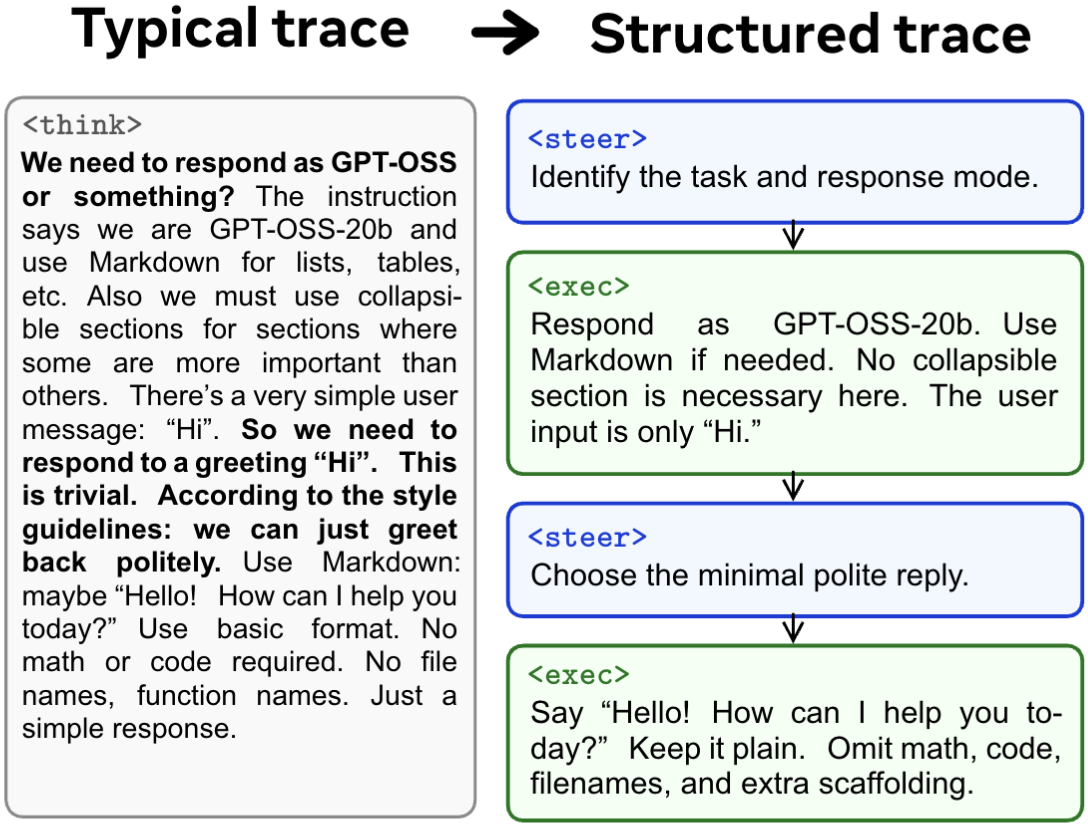
\includegraphics[width=\columnwidth]{assets/typical_vs_structured.png}
  \caption{\emph{Left}. A partial reasoning trace generated by OpenAI's
    \texttt{GPT-OSS-20B} in response to ``Hi''. It mixes strategy selection and
    execution in one long token stream. \emph{Right}. The
    \methodname{} format separates short \texttt{<steer>} decisions
    from longer \texttt{<exec>} spans, creating explicit control points for inspection, branching, and credit assignment.}
  \label{fig:typical-vs-structured}
\end{figure}

The options framework of \citeauthor{sutton1999between} is the natural reference point for
\methodname{}: it lets an agent choose temporally extended actions rather
than primitive actions, turning a flat MDP into a semi-MDP over higher-level
moves. Later hierarchical RL systems such as h-DQN and option-critic explicitly split
the high-level policy from the lower-level policy \cite{kulkarni2016hdqn,bacon2017optioncritic}. Although
intriguing, we do not train separate models or use Q-learning over strategy-level
options. Language models already operate across the hierarchy of abstraction.
\methodnamestart{} simply delineates this alternating hierarchy with
\texttt{<steer>} and \texttt{<exec>} XML blocks.

\citeauthor{wang2025eightyentropy}'s `80/20' result provides a useful existence proof:
high-entropy minority tokens act as ``forking tokens,'' and restricting
RL updates to roughly the top 20\% of tokens can match or outperform full-token
updates. That finding supports the idea that
reasoning traces contain sparse decision points; however, the mechanism of high-entropy
tokens remains opaque. \methodnamestart{} makes the decision point explicit in
the trace, so exploration can sample directly from a strategic action space rather than
an arbitrary next token. We find that \texttt{<steer>} decision tokens are
consistently in the top 95th percentile for entropy, making them good targets under the
`80/20' rule for credit assignment.

Methods for credit assignment range from naïve outcome-only rewards with
undifferentiated per-token advantage scores to dense rewards via process supervision
and process reward models (PRM) \cite{uesato2022process,lightman2023verify}. Tree methods identify
advantageous actions during policy
optimization by branching rollouts from shared prefixes and comparing the downstream
value of alternative continuations \cite{treepo2025,treegrpo2025,tempo2025,treerl2025}.
An emphasis on boundaries is present throughout credit assignment work.
\citet{lightman2023verify} train reward models to score newline-delimited reasoning
steps. Many later systems keep pragmatic text-level step conventions: recent PRM work
prefers paragraph-end \verb|\n\n| tokens as step separators
\cite{zheng2025processbench,zhang2025prmlessons}. \methodnamestart{} makes these boundaries
intuitive: a \texttt{<steer>} block isolates high-level decisions---perfect
for tree branching. When paired with its \texttt{<exec>} block, the
interleaving
\texttt{<steer>}/\texttt{<exec>} structure is well-matched for
PRM step decompositions.

Recent RL work on LLM exploration highlights how high-temperature rollouts produce
mostly surface variation with few strategically unique rollouts. DIVER and Meta's
DARLING treat diversity as an RL objective, rewarding responses that are
both high quality and semantically distinct \cite{hu2025diver,li2025darling}. Other
work asks where extra samples should be spent, using semantic coverage or
uncertainty-triggered branching rather than uniform high-temperature full-trajectory
sampling \cite{ets2025,fr3e2025,arpo2025}. \methodnamestart{}'s structure
allows high-temperature sampling to be focused on key decision points. We make the
design choice to limit high-level decisions to 15 tokens, enabling efficient sampling
of the policy's distribution over the next high-level decision for search and
up-weighting of rare strategies.

During the design of the \methodname{} dataset, we found that the model
lacked any ability to follow out-of-distribution (OOD), off-policy decisions
inserted into the middle of a reasoning trace. CoT-Control shows that reasoning models
struggle to control the content of their own chains of thought, especially compared
with their final outputs \cite{chen2026controlcot}. \citeauthor{vonrecum2026cotrobust} find
that reasoning models are robust to perturbations inserted into their reasoning,
effectively ignoring disruptions by doubting them; however, they argue this behavior is
desirable. Intervening and controlling reasoning behavior remains poorly understood.
Viewed through the lens of MDP design, training with imprecise, high-temperature,
token sampling necessitates strong robustness against research-induced token noise.
We assert that treating reflexive doubt \cite{vonrecum2026cotrobust,muennighoff2025s1} as the `modus
operandi'
of reasoning is a shortcoming. To improve intra-reasoning faithfulness to
both on- and off-policy steering, \methodname{}'s dataset includes
examples of faithfulness to intervening commands.

\section{Problem Setup}
\label{sec:problem-setup}

Let \(x^{\mathrm{in}} \in \mathcal{X}\) denote a
problem prompt drawn from a
distribution
\(\mathcal{D}\), and let
\(x^{\mathrm{out}} =
(a_1,\ldots,a_T)\)
denote the full completion sampled from an
autoregressive language model \(\pi_\theta\). A task verifier provides a
terminal reward \(R(x^{\mathrm{in}},x^{\mathrm{out}})
\in [0,1]\), usually by extracting the final
answer
from \(x^{\mathrm{out}}\). The standard token-level view is an MDP in
which the state is the
current prefix \(s_t =
(x^{\mathrm{in}},a_{<t})\), the action
is the next token
\(a_t\), the transition appends \(a_t\) to the
prefix, and the reward is
observed only after the final token.

\begin{equation}
  \begin{aligned}
    p_\theta(x^{\mathrm{out}} \mid x^{\mathrm{in}})
     & =
    \prod_{t=1}^{T} \pi_\theta(a_t \mid x^{\mathrm{in}},a_{<t}), \\
    J_{\mathrm{tok}}(\theta)
     & =
    \mathbb{E}_{x^{\mathrm{in}} \sim \mathcal{D}}
    \mathbb{E}_{x^{\mathrm{out}} \sim \pi_\theta(\cdot \mid x^{\mathrm{in}})}
    [R(x^{\mathrm{in}},x^{\mathrm{out}})].
  \end{aligned}
  \label{eq:token-mdp}
\end{equation}

This representation is exact, but it exposes the wrong control surface for
long reasoning: the horizon is \(T\), the actions are tokens, and the useful
semantic decisions are implicit inside prefixes.

\methodnamestart{} keeps the same underlying task and model, but changes the
representation of the reasoning trace. A valid trace is parsed into
\(K\) decision--execution pairs,
\begin{equation}
  x^{\mathrm{out}} =
  (o_1,b_1,\ldots,o_K,b_K),
  \label{eq:basic-trace}
\end{equation}
where each \(o_k\) is the text inside a \texttt{<steer>} span and each
\(b_k\) is the text inside the following \texttt{<exec>} span. The intended
regime is \(|o_k| \ll |b_k|\): in our data, steering spans are short
natural-language decisions, while execution spans contain the longer reasoning
needed to carry out those decisions. Let
\(z_k = (x^{\mathrm{in}},o_1,b_1,\ldots,o_{k-1},b_{k-1})\) be the
prefix before the
\(k\)-th decision. The same language model then induces two conditional
distributions:
\begin{equation}
  p_\theta(x^{\mathrm{out}} \mid x^{\mathrm{in}})
  =
  \prod_{k=1}^{K}
  \pi_\theta^{\mathrm{steer}}(o_k \mid z_k)
  \pi_\theta^{\mathrm{exec}}(b_k \mid z_k,o_k).
  \label{eq:basic-factorization}
\end{equation}
These are not separate networks or an external planner. They are the
conditional distributions of the same autoregressive model under the
\methodname{} format.

This factorization induces a semi-MDP over reasoning steps. The high-level
state is \(z_k\), the high-level action is the steering decision \(o_k\), and
the execution \(b_k\) is the transition to
\(z_{k+1} = (z_k,o_k,b_k)\). Equivalently,
\begin{equation}
  P_\theta(z_{k+1} \mid z_k,o_k)
  =
  \sum_{b:\, z_{k+1}=(z_k,o_k,b)}
  \pi_\theta^{\mathrm{exec}}(b \mid z_k,o_k).
  \label{eq:basic-transition}
\end{equation}
The terminal reward remains
\(R(x^{\mathrm{in}},x^{\mathrm{out}})\), but the
effective decision horizon is
\(K\) rather than \(T\). The central question in this report is whether this
representation preserves task performance while providing better handles for
exploration, credit assignment, interpretation, and intervention.

\begin{center}
  \centering
  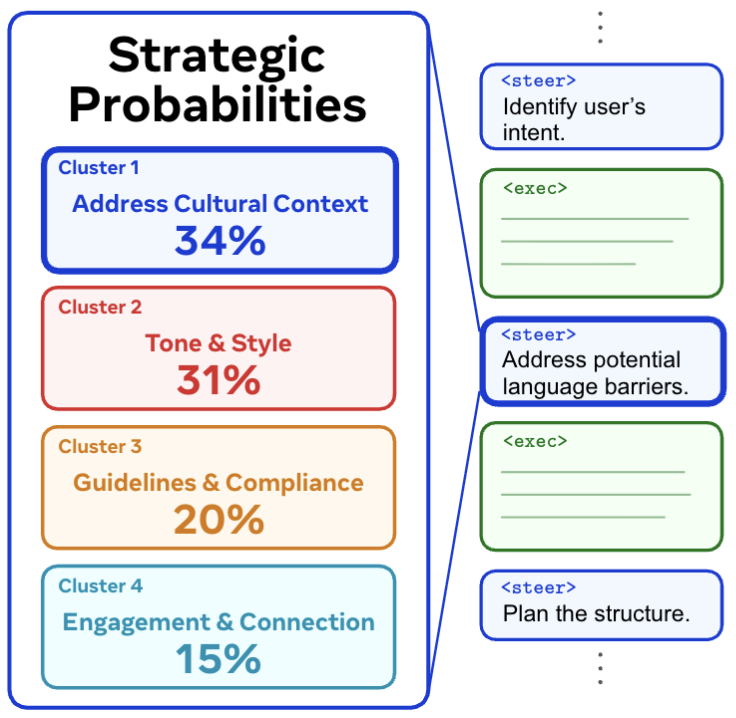
\includegraphics[width=\columnwidth]{assets/strategic-probabilities.png}
  \captionsetup{hypcap=false}
  \captionof{figure}{A \texttt{<steer>} boundary makes the model's next-step
    strategy distribution interpretable: many sampled decisions can be grouped
    into semantic modes, revealing which high-level options the model is
    considering before it commits to an execution path.}
  \label{fig:strategic-probabilities}
\end{center}

\subsection{Data}
\label{sec:data}

The SFT dataset is designed to teach the \methodname{} representation. We
start by sampling rows from OLMo 3's \emph{Dolci-Think-SFT-7B} dataset, a warm-up
reasoning dataset whose assistant messages contain \texttt{<think>...</think>} traces
\cite{allenai2026dolcithinksft7b}. From this base, we keep examples up to 16,328 tokens:
we found very long traces lose coherence and are difficult to rewrite into the
\methodname{} format without additional scaffolding. We also stratify
across domains so that the dataset is balanced.

Each reasoning trace is rewritten into the \methodname{} format by
converting
the original \texttt{<think>} block into alternating
\texttt{<steer>} and
\texttt{<exec>} spans. We prompt a larger model to add the structure,
instructing
it to stay close to the original reasoning, split only when the solution process
changes direction, keep steering commands terse, and leave the detailed work in
execution blocks. The goal is to expose the latent hierarchy already
present in the original trace. We therefore keep only transformed rows whose
traces are structurally valid (interleaved and correctly closed
\texttt{<steer>}
and \texttt{<exec>} tags) and whose length remains close to the source
trace to
avoid excessive mutation.

We found during initial research that the model is much more likely to follow
\texttt{<steer>} commands that are generated by its own policy rather than
off-policy interventions. This behavior is consistent with \citet{vonrecum2026cotrobust},
who find that reasoning models often recover from or dampen interventions inserted
into their own chain of thought.

To improve controllability, we modify 25\% of the transformed data with interventions.
These interventions add curated \texttt{<steer>}/\texttt{<exec>}
spans
(1-3 pairs) at random locations within the reasoning trace. The trace still alternates
correctly. We generate these interventions by prompting a larger model to follow
specific \texttt{<steer>} commands along with the prefix at the insertion
point.
We insert two types of interventions: meta-cognitive
reflections, motivated by cognitive-foundations work that treats
self-monitoring and strategy selection as central reasoning controls
\cite{kargupta2025cognitivefoundations}, and random non-sequiturs. All interventions can be
universally applied to any domain of reasoning.

\textbf{Meta-cognitive} interventions ask the model to reflect on its own
reasoning. For example:

\begin{center}
  ``\texttt{<steer>}Summarize progress so far\texttt{</steer>}''
  ``\texttt{<steer>}Imagine this approach fails\texttt{</steer>}''
  ``\texttt{<steer>}List 5 alternative approaches\texttt{</steer>}''
\end{center}

\textbf{Non-sequitur} interventions ask the model to follow a command that is not
aligned with the task. For example:

\begin{center}
  ``\texttt{<steer>}Give the current task a
  nickname\texttt{</steer>}''
  ``\texttt{<steer>}Express emotions about the
  task\texttt{</steer>}''
  ``\texttt{<steer>}Make NASA stand for snacks\texttt{</steer>}''
\end{center}

We use a judge prompt to determine if the original reasoning traces can be continued
without modification after an intervention. If a reasoning trace needs
modification, we regenerate it using OLMo 3 7B SFT trained to follow the
\methodname{} format.

The two types of interventions used in the \methodname{} dataset are
designed
to train faithfulness to \texttt{<steer>} commands at any point in the
reasoning process. Meta-cognitive interventions remain task-aligned
while the non-sequitur interventions are task-disruptive. To avoid learning a
task-disruptive high-level steering policy, we mask non-sequitur
\texttt{<steer>} tokens during SFT, training only for faithfulness in
the \texttt{<exec>} blocks. Together with the reasoning-derived
\texttt{<steer>}/\texttt{<exec>} pairs, these interventions
create a continuum of task-alignment for \texttt{<steer>} commands, teaching
the model to follow them even when they are not helpful.

The final SFT dataset contains 2,193 conversations. The main domains covered are
science, Python code, mathematics, multilingual chat, and instruction-following.
The source Dolci dataset is licensed under ODC-BY for research and educational use.

\subsection{Metrics}
\label{sec:metrics}

We evaluate reasoning performance using the American Invitational Mathematics
Examination (AIME) '24/'25 benchmarks. Each year's AIME competition contains
30 problems. Answers are integers between 0 and 999. We extract
\verb|\boxed{}|
answers from the output and compare them by exact match with the ground truth answers.

We check for repeated reasoning traces, terminate them early, and cut generation off
at 32,768 tokens. We report average per-problem pass rate.

(Draft: Not Implemented Yet)
\begingroup
\color{red!80!black}
To measure the faithfulness of \texttt{<exec>} blocks to
\texttt{<steer>} decisions, we use a judge model prompted with a
faithfulness
rubric. We sample various \texttt{<steer>}/\texttt{<exec>} pairs
from
AIME '24/'25 rollouts that follow on-policy and off-policy steering commands at
different depths in the reasoning chain.
\par
\endgroup

\section{Method}
\label{sec:method}

We first cover the method used to train the \texttt{<steer>}
/\texttt{<exec>} format via SFT. Subsequently, to
realize the full benefit of the \methodname{} decomposition, we pair
training with a
structured decoder to isolate high-level sampling, \(\pi_\theta^{\text{steer}}\),
from low-level sampling, \(\pi_\theta^{\text{exec}}\). With
\texttt{<steer>} spans independently sampled, we can
effectively apply classic RL methods for exploration, credit assignment, and data
efficiency. We experiment with \(\varepsilon\)-greedy exploration and basic tree
search. (Draft: Not Implemented Yet)
\begingroup
\color{red!80!black}
Lastly, we evaluate intra-CoT faithfulness to ascertain the deference
given to \texttt{<steer>} decision spans by the low-level execution policy,
\(\pi_\theta^{\text{exec}}\).
\endgroup

\begin{table*}[t]
  \centering
  \small
  {%
    \renewcommand{\tabularxcolumn}[1]{b{#1}}%
    \begin{tabularx}{0.9\textwidth}{@{}c >{\raggedright\arraybackslash}p{0.05\textwidth} X >{\raggedright\arraybackslash}b{0.11\textwidth}@{}}
      \toprule
      Step               & Mode          & Completion                                                                                                                                                                                      & Append                       \\
      \midrule
      \multirow{2}{*}{1} & High          & Split problem into cases\steertag{</steer}\stoptag                                                                                                                                              & \steertag{>}\exectag{<exec>} \\
                         & \lowmodelabel & Let's split this problem into 2 cases, \(a < 0\), \(a \geq 0\). I'll start with case 1 ... so case 1 holds\exectag{</exec>}\steertag{<steer}\stoptag                                            & \steertag{>}                 \\
      \midrule
      \multirow{2}{*}{2} & High          & Check case 2\steertag{</steer}\stoptag                                                                                                                                                          & \steertag{>}\exectag{<exec>} \\
                         & \lowmodelabel & Case 2 is \( a \geq 0 \). When this is the case, the algebra works out differently. Let's see... so the result holds for \(a>0\) but not for \(a=0\).\exectag{</exec>}\steertag{<steer}\stoptag & \steertag{>}                 \\
      \midrule
      \multirow{2}{*}{3} & High          & Double check a=0 case\steertag{</steer}\stoptag                                                                                                                                                 & \steertag{>}\exectag{<exec>} \\
                         & \lowmodelabel & When a=0, we have f(x) / 0, which is undefined, so let's analyze the limits again... how interesting that\budgettag                                                                             & \exectag{</exec>}            \\
      \midrule
      \multirow{2}{*}{4} & High          & \steertag{<steer>}Summarize Final Answer\steertag{</steer}\stoptag                                                                                                                              & \steertag{>}\exectag{<exec>} \\
                         & \lowmodelabel & Putting it all together, the \(a=0\) exception is invalid, so the final answer is 42.\exectag{</exec>}\texttt{</think>}The answer is \texttt{\textbackslash boxed\{}42\texttt{\}}\eos           &                              \\
      \bottomrule
    \end{tabularx}
    \caption{
      Illustrative structured decoding trace. Each reasoning step is composed of high- and
      low-level completions. In total, this uses 8 API calls to vLLM, one for each \texttt{<steer>} or \texttt{<exec>} completion.
      Red bracketed text signifies the stop reason. Completion modes that reach \budgettag
      are
      forced to hand off
      token generation by appending the closing XML tag to the interrupted token stream.
    }
    \label{tab:structured-decoding-example}
  }%
\end{table*}

\subsection{Masked Supervised Learning}
\label{sec:masked-supervised-learning}

Given a transformed conversation \((x_i^{\mathrm{in}},\tau_i)\), where
\(\tau_i=(o_1,b_1,\ldots,o_K,b_K)\) is the assistant reasoning trace in the
\methodname{} format, we fine-tune the base model with next-token
prediction on
the assistant completion. Let \(\tau_{i,t}\) be the \(t\)-th target
token and
let \(m_{i,t}\in\{0,1\}\) indicate whether that token is
supervised. The SFT
objective is
\begin{equation}
  \mathcal{L}_{\mathrm{SFT}}(\theta)
  =
  -\frac{
    \sum_i \sum_t m_{i,t}
    \log \pi_\theta(\tau_{i,t}\mid x_i^{\mathrm{in}},\tau_{i,<t})
  }{
    \sum_i \sum_t m_{i,t}
  }.
  \label{eq:sft-loss}
\end{equation}
For ordinary transformed traces, \(m_{i,t}=1\) for all
assistant tokens. For non-sequitur intervention traces, we mask the inserted
non-sequitur \texttt{<steer>} decision tokens but leave the corresponding
\texttt{<exec>} tokens supervised. This trains the model to obey an
arbitrary steering command when it appears in the context, without training the model
to choose task-irrelevant commands as its own high-level policy.

All training examples are required to parse as an alternating sequence of
\texttt{<steer>} and \texttt{<exec>} spans inside the
\texttt{<think>} block. Invalid traces are filtered
before training. The result is a standard causal language model whose output can be
parsed into the factorization in equation~\ref{eq:basic-factorization}.

We train \texttt{Qwen3-8B} \citep{qwen3_2025} and
\texttt{Olmo-3-7B-Think-SFT} \citep{olmo2025olmo3} using this masked
SFT procedure with Hugging Face's TRL framework \citep{vonwerra2020trl}. We conduct
full-parameter bf16 fine-tuning for 8 epochs on packed sequences with a 16K token
length
on a single node with 4\(\times\) NVIDIA A100-SXM4-80GB GPUs on the Ohio Supercomputer
Center's Ascend Cluster. With DeepSpeed ZeRO stage 2
\citep{rasley2020deepspeed,rajbhandari2020zero}, training takes 1.5 hours and maintains 99.0\% average GPU
utilization with peak VRAM consumption at 96.7\% (average of 90.1\%).

\subsection{Structured Decoding}
\label{sec:structured-decoding}

At inference time, we use the model's normal chat template and ask it to produce
a \texttt{<think>} trace. Block generation proceeds normally until the model
either finishes, reaches the token budget, or ends its chunk with
\texttt{</steer>} or \texttt{</exec><steer>}. To keep the process
append-only and avoid deleting tokens from the generated sequence, we use partial XML
tags \texttt{"</steer"} and \texttt{"<steer"} as stop sequences in
vLLM \cite{kwon2023pagedattention} (not \texttt{"</exec"} since the model may
choose \texttt{"</exec></think>"}). For high-level decision blocks, we set a token
budget of 15. For low-level execution, we set a per-block
token budget of 512. Both high- and low-level budgets cover over 99\% of training
data. When block generation terminates, we check the tail of the token sequence for any
prefix of \texttt{</steer><exec>} or \texttt{</exec>} and enforce
complete boundary XML. We do not force \texttt{</exec><steer>} since the model may
prefer to \emph{terminate} generation with \texttt{</exec></think>}.

We complete XML tags and concatenate decision and execution blocks in
token-space to avoid repeated re-tokenization issues \cite{xu2026partialtoken}.

With each block as an independent vLLM API call, we take care
to avoid evicting KV cache for in-flight long CoT traces. The vLLM inference engine
evicts KV cache for old or queued requests when GPU memory cannot fit the additional
cache for running requests. To mitigate KV cache thrashing, we limit concurrently
running rollouts with a conservative async semaphore and consistent queue ordering
using priority queue mechanics available in vLLM. KV cache thrashing can reduce
generation speed from hundreds of tokens per second to tens of tokens per second.

This procedure keeps every generated completion structurally valid while making the
short decision, \(o_k\), and sampling method over the steering policy
\(\pi_{\theta}^{\text{steer}}\),
distinct and easy to customize. For example, sampling from the steering policy,
\(\pi_{\theta}^{\text{steer}}\),
can use a higher temperature for high-level-only exploration:
$$
  \text{Temperature}_{\text{steer}}>\text{Temperature}_{
  \text{exec}}
$$

\subsection{\headvarepsilon-Greedy Exploration}
\label{sec:decision-point-exploration}

We experiment with exploration techniques enabled by \methodname{}'s
structured decoder.
We replace token-wise high-temperature sampling with oversampling
at the \texttt{<steer>} boundary.

Figure~\ref{fig:epsilon-greedy-exploration} summarizes the decision-point
\(\varepsilon\)-greedy exploration setup.

Specifically, inspired by \(\varepsilon\)-greedy exploration
\citep{sutton2018reinforcement}, we use a custom on-policy branch that invokes
Algorithm~\ref{alg:decision-point-epsilon} with probability \(\varepsilon\);
otherwise it samples a normal steering completion. The procedure is as follows:

\begin{enumerate}
  \item Sample \(n=100\) \texttt{<steer>} completions at
        \(\mathrm{temp}=1\) and \texttt{token\_budget=15}.
  \item Build either semantic clusters or an embedding-diverse shortlist.
  \item Sample a \texttt{<steer>} completion from the selected cluster or
        diverse shortlist.
  \item Append the selected candidate as \(o_k\) and continue with structured
        decoding.
\end{enumerate}

\begin{figure*}[t]
  \centering
  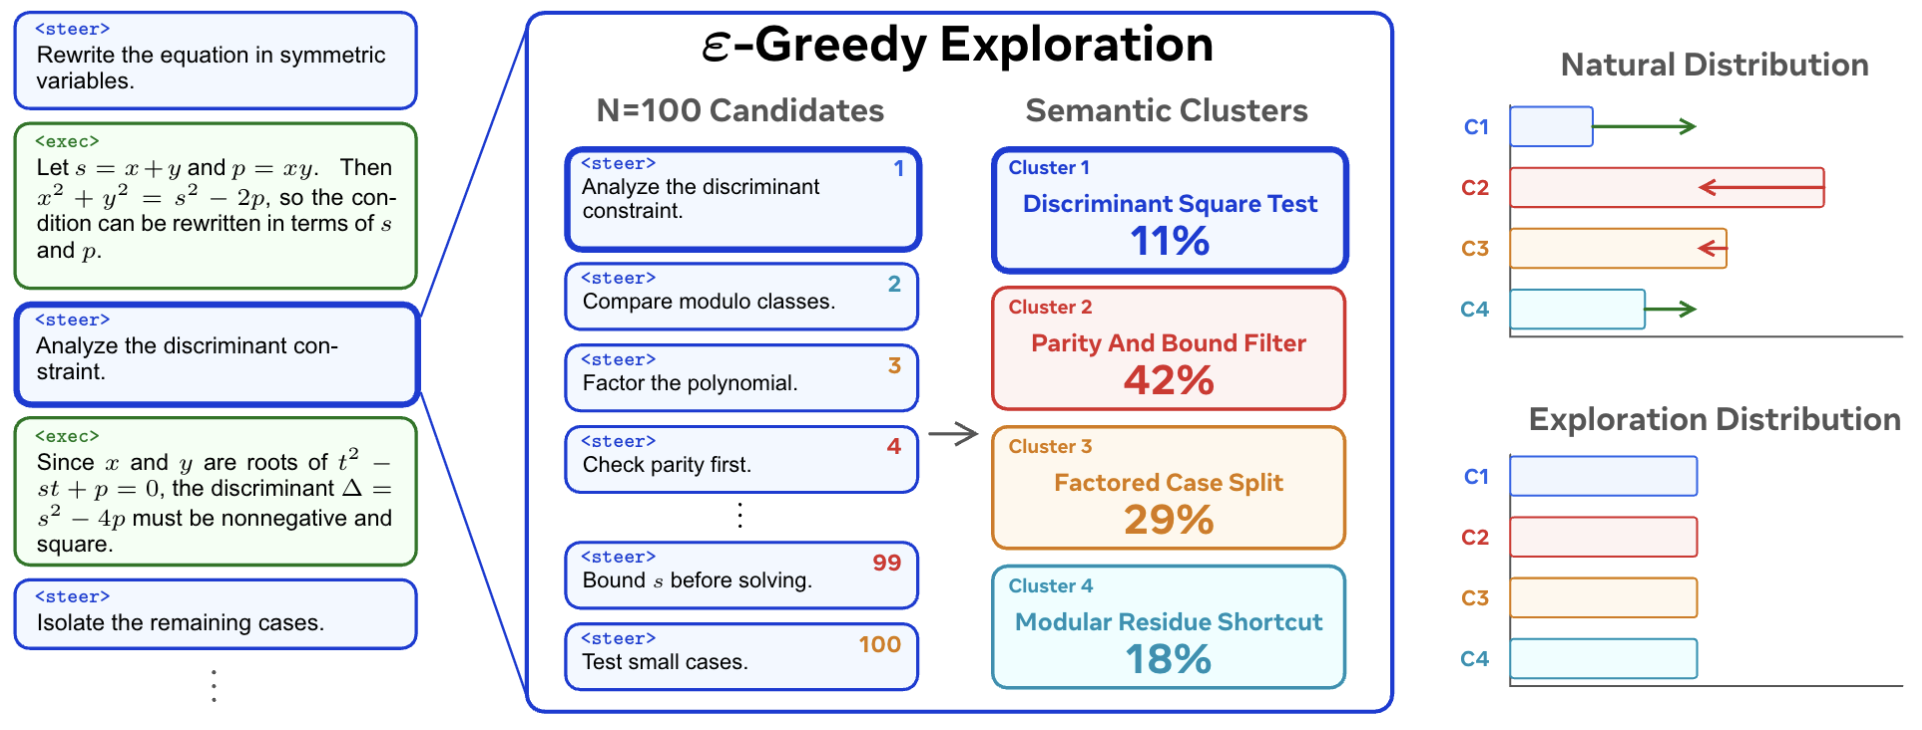
\includegraphics[width=\textwidth]{assets/Eps-Greedy-Figure.png}
  \caption{Decision-point \(\varepsilon\)-greedy exploration samples many
    candidate \texttt{<steer>} actions at a boundary, groups them into semantic
    modes, and selects from the induced exploration distribution rather than
    only following the model's natural next-decision distribution. This approach upsamples
    rare reasoning strategies and escapes modal behaviors.}
  \label{fig:epsilon-greedy-exploration}
\end{figure*}

Because \texttt{<steer>} decisions are shorter than 15 tokens each,
oversampling 100 candidates in parallel remains computationally and memory efficient.
Oversampling enables on-policy exploration when rare semantic modes can be upsampled.
For example, consider that when prompted merely with "Hello", reasoning models tend to
overthink their responses. Using \texttt{Qwen3-8B} trained on the
\methodname{} dataset, we sampled and clustered 100 candidate steering
decisions
after the fourth \texttt{<steer>} span and 176 thinking tokens into
reasoning about
``Hello''. Clustering identified 8 different high-level options
the model was considering as the next step in its reasoning:

\begin{table}[H]
  \centering
  \begin{tabular}{r l}
    \hline
    Count        & Action                            \\
    \hline
    23\(\times\) & Re-Analyze Context and Intent     \\
    22\(\times\) & Verify Against Guidelines         \\
    21\(\times\) & Refine and Polish                 \\
    12\(\times\) & Consider Cultural/Language Nuance \\
    11\(\times\) & Decide on Style or Tone           \\
    6\(\times\)  & Finalize Response                 \\
    4\(\times\)  & Brainstorm Alternatives           \\
    1\(\times\)  & ``Reflect on the Role of AI''     \\
    \hline
  \end{tabular}
\end{table}

Oversampling at decision boundaries provides highly intuitive interpretability by
contextualizing reasoning within the space of unselected alternate possibilities.
In this example, 94\% of rollouts would have continued overthinking the response.
\(\varepsilon\)-greedy exploration doubled the probability of the ``Finalize
Response'' option from 6\% to 12.5\%. We are happy to report that the model finally
said ``hello'' back.

\subsection{Tree Search}

Although more sophisticated approaches exist for tree search, we wanted to
understand the utility of the \methodname{} structure for identifying
meaningful step boundaries and branch points. We therefore test a deliberately
simple tree-search method using Algorithm~\ref{alg:decision-point-epsilon} as
the candidate selector. At each branchable \texttt{<steer>} boundary, we
sample a small set of short steering candidates. We then choose multiple candidates
without replacement. Similar to Algorithm~\ref{alg:decision-point-epsilon}, we
emphasize diversity using clustering or, more directly, diversity-based sampling.

We note that the branch trigger need not be random. TreeRL shows that tree
search is more efficient when branching is triggered by the highest entropy tokens in a
reasoning trace \citep{treerl2025}. \methodnamestart{}
offers a natural version of the same idea at the level of reasoning strategies.
At a \texttt{<steer>} boundary, many short candidate decisions can be
sampled and clustered into semantic modes. Aggregating candidate
mass within each cluster gives an empirical distribution from which entropy can be
computed and used for opportune branching.

Each selected steering command becomes a child branch by appending the selected
text, closing the steering span, and opening the execution span. The branch then
decodes execution tokens until the next \texttt{<steer>} boundary or
termination. We continue over the frontier until the leaf budget is reached or a
path has used its branch-point budget; after that, the path continues with
ordinary structured decoding.

Tree-based rollout structures work well with vLLM's KV-cache machinery
\cite{kwon2023pagedattention}. With paged KV cache blocks and prefix caching, the shared
prefix can be reused while child branches allocate cache for only the diverging suffix.

\subsection{Intervention Evaluation}
\label{sec:intervention-evaluation}

WIP

\subsection{Reinforcement Learning}
\label{sec:reinforcement-method}

(Draft: WIP)
\begingroup
\color{red!80!black}
The planned reinforcement-learning phase will train \methodname{} models
on
\texttt{allenai/Dolci-Think-RL-7B} \citep{allenai2026dolcithinkrl7b} using
DAPO \citep{yu2025dapo}. The intended comparison is between ordinary
response-level RL and a structured variant that treats \texttt{<steer>}
boundaries as higher-level decision points for credit assignment and exploration.
This experiment is not yet complete.
\par
\endgroup

\section{Results}
\label{sec:results}

We report partial results for the class project in
Tables~\ref{tab:aime-results} and~\ref{tab:epsilon-ablation}. These runs are
intended to show whether the \methodname{} interface preserves baseline
reasoning performance and whether structured decoding can expose useful
test-time exploration knobs. Entries marked WIP are still incomplete.

\begin{table}[h]
  \centering
  \caption{AIME accuracy for base models and \methodname{} decoding variants.
    Pass rate is averaged over 32 rollouts.}
  \label{tab:aime-results}
  \small
  \begin{tabularx}{\columnwidth}{>{\raggedright\arraybackslash}Xcc}
    \toprule
    Model                                    & AIME '24 & AIME '25 \\
    \midrule
    \texttt{Qwen3-8B}                        & 76.00\%  & 67.30\%  \\
    + \methodname{}                          & WIP      & WIP      \\
    + \methodname{} + \(\varepsilon\)-Greedy & WIP      & WIP      \\
    + \methodname{} + Tree                   & 76.72\%  & WIP      \\
    + \methodname{} + Tree + Clustering      & 77.30\%  & WIP      \\
    \midrule
    \texttt{OLMo3-7B-Think-SFT}              & 69.60\%  & 57.60\%  \\
    + \methodname{}                          & 63.95\%  & 51.56\%  \\
    + \methodname{} + \(\varepsilon\)-Greedy & 64.33\%  & 52.70\%  \\
    + \methodname{} + Tree                   & 63.13\%  & 46.01\%  \\
    + \methodname{} + Tree + Clustering      & 63.28\%  & 48.54\%  \\
    \bottomrule
  \end{tabularx}
\end{table}

The current pattern is mixed. On Qwen3-8B, tree search gives a small preliminary
gain on AIME '24, especially when steering candidates are clustered before
branching, but AIME '25 runs remain unfinished. On OLMo3-7B-Think-SFT, the
\methodname{} SFT model trails the original checkpoint on aggregate AIME
pass rate, while \(\varepsilon\)-greedy decoding modestly improves over vanilla
\methodname{} decoding. The per-problem ablation also suggests that
exploration is highly sensitive to the problem and exploration rate:
\(\varepsilon=33\%\) helps one OLMo problem but not another, and \(\varepsilon=66\%\)
can reduce pass rate. Tree-based pass rates are also difficult to estimate
cleanly because leaves from the same tree share long correlated prefixes, which
can make aggregate pass-rate estimates high variance across evaluation runs. One
interesting observation is that early termination due to repetition occurs at much
higher rates with
OLMo3-7B-Think-SFT than for Qwen3-8B on the sampled problems, suggesting that
the structured decoder interacts differently with each base model's tendency to
loop. These trends motivate better evaluation of controllability and diversity
rather than relying only on final-answer accuracy.

\begin{table}[h]
  \centering
  \caption{\(\varepsilon\)-greedy pass rates and repetition rates on selected
    AIME '25 problems for \methodname{} models.}
  \label{tab:epsilon-ablation}
  \scriptsize
  \setlength{\tabcolsep}{3pt}
  \begin{tabularx}{\columnwidth}{@{}>{\raggedright\arraybackslash}Xcccc@{}}
    \toprule
                           & \multicolumn{2}{c}{Pass Rate} & \multicolumn{2}{c}{Repetition Rate}                     \\
    \cmidrule(lr){2-3}\cmidrule(l){4-5}
    Setting                & \#6                           & \#12                                & \#6     & \#12    \\
    \midrule
    \multicolumn{5}{l}{\texttt{OLMo3-7B-Think-SFT} + \methodname{}}                                                  \\
    \(\varepsilon\) = 0\%  & 17.19\%                       & 2.08\%                              & 13.02\% & 15.10\% \\
    \(\varepsilon\) = 33\% & 18.30\%                       & 0.00\%                              & 10.27\% & 16.33\% \\
    \(\varepsilon\) = 66\% & 14.58\%                       & 0.00\%                              & 12.50\% & 25.17\% \\
    \midrule
    \multicolumn{5}{l}{\texttt{Qwen3-8B} + \methodname{}}                                                            \\
    \(\varepsilon\) = 0\%  & 31.25\%                       & 2.08\%                              & 2.60\%  & 2.60\%  \\
    \(\varepsilon\) = 33\% & WIP                           & WIP                                 & WIP     & WIP     \\
    \(\varepsilon\) = 66\% & 28.13\%                       & 0.52\%                              & 1.56\%  & 1.04\%  \\
    \bottomrule
  \end{tabularx}
\end{table}

\section{Limitations and Next Steps}
\label{sec:limitations-next-steps}

The main limitation of the current evaluation is that AIME accuracy is a blunt
measure of the mechanism we are trying to study. The project is about
turning reasoning into a steerable high-level policy and a lower-level execution
policy, but final-answer pass rate only observes the end of the trajectory. It
does not tell us whether the model followed a supplied \texttt{<steer>}
decision, whether branching explored genuinely different strategies, or whether a
failure came from choosing the wrong strategy versus executing a good strategy
poorly.

A better measurement target is faithfulness to interventions. Given a prefix and
an inserted \texttt{<steer>} decision, we can measure whether the following
\texttt{<exec>} span actually carries out that decision under both
on-policy and
off-policy commands. This directly tests the contract that makes
\methodname{} useful as a control interface.

Evaluation should also include distributional diversity benchmarks such as
NoveltyBench \citep{zhang2025noveltybench}. Since \(\varepsilon\)-greedy
sampling and branching are meant to reveal alternate reasoning modes, a benchmark
that scores distinct, high-quality generations is a better match than a single
best-answer metric alone.

Ultimately, however, the method is a redesign of the MDP for RLVR. To evaluate the
effect, we need to run RL training. The planned run is to train on
\texttt{allenai/Dolci-Think-RL-7B} with DAPO
\citep{allenai2026dolcithinkrl7b,yu2025dapo}, then compare ordinary
response-level updates against updates that exploit \texttt{<steer>}
boundaries
for credit assignment, exploration, and possibly entropy-triggered branching.
That would test whether the structure improves learning rather than just test-time
sampling behavior.

\section{Conclusion}
\label{sec:conclusion}

RLVR has largely relied on
treating generation as a flat, token-level decision process. In this report, we
challenged this minimal default formulation by introducing BASIC, an approach that
reorganizes long-form reasoning into a hierarchical Markov decision process. By
strictly alternating between short, high-level strategic decisions and longer,
low-level executions, BASIC provides a more natural abstraction for both the model and
the researcher.

Our preliminary experiments demonstrate that models can be effectively fine-tuned to
adopt this decomposed reasoning structure without sacrificing baseline performance on
rigorous benchmarks such as AIME '24 and '25. More importantly, this structure exposes
a
highly interpretable and manipulable control surface. By decoupling strategy from
execution, we enable targeted test-time interventions, such as
\(\varepsilon\)-greedy exploration and tree search, directly at discrete
decision boundaries. As observed in our sampling clusters, these methods can
successfully upsample rare, semantically distinct reasoning modes, helping to bypass
the modal behaviors and entropy collapse typical of unstructured high-temperature
sampling.

While final-answer accuracy serves as a sanity check during the SFT phase, the true
promise of the BASIC framework lies in its potential to
resolve the credit assignment and exploration bottlenecks inherent to RLVR. By
isolating high-impact strategic tokens from execution-heavy spans, this structure lays
the necessary groundwork for our upcoming reinforcement learning phase. Ultimately,
structuring long chain-of-thought into explicit, steerable horizons offers a principled
path toward reasoning models that do not merely execute prior behaviors more reliably,
but genuinely explore and discover novel problem-solving strategies.

\section*{Acknowledgments}
This work used resources from the Ohio Supercomputer Center.

\clearpage
\bibliographystyle{plainnat}
\bibliography{references}

\clearpage
\appendix
\section*{Appendix}
\section{Decision-Point Exploration Algorithm}
\label{app:decision-point-exploration-algorithm}

\begin{algorithm}[H]
  \caption{Decision-point \(\varepsilon\)-greedy steering}
  \label{alg:decision-point-epsilon}
  \small
  \begin{minipage}{\linewidth}
    \textbf{Input:} prefix
    \(z_k\texttt{<steer>}\), policy
    \(\pi_\theta^{\mathrm{steer}}\), exploration rate \(\varepsilon\),
    candidate count \(N=100\), selector \(\sigma\in
    \{\mathrm{cluster},\mathrm{diverse}\}\), shortlist cap
    \(M=20\).\\
    \textbf{Helper:} \(S(z;T,B)\) samples one steering candidate from
    \(\pi_\theta^{\mathrm{steer}}(\cdot\mid z)\) with temperature \(T\), budget
    \(B\), and stop sequence \texttt{</steer>}.\\
    \textbf{Return:} \(\operatorname{Complete}(z,o)=
    z\,o\,\texttt{</steer><exec>}\).

    \begin{tabbing}
      \quad\=\quad\=\quad\=\kill
      \(r \leftarrow \operatorname{Uniform}(0,1)\)\\
      \textbf{if} \(r > \varepsilon\) \textbf{then}\\
      \> \(o_k \leftarrow S(z_k;T_{\mathrm{base}},15)\)\\
      \> \textbf{return} \(\operatorname{Complete}(z_k,o_k)\)\\
      \textbf{end if}\\[0.2em]
      \(C_k \leftarrow \emptyset\)\\
      \textbf{for} \(i=1,\ldots,N\) \textbf{do}\\
      \> \(c_i \leftarrow S(z_k;1,15)\)\\
      \> \(C_k \leftarrow C_k \cup \{\operatorname{StripTags}(c_i)\}\)\\
      \textbf{end for}\\[0.2em]
      \(D_k \leftarrow \operatorname{Deduplicate}(C_k)\)\\
      \textbf{if} \(\sigma=\mathrm{cluster}\)
      \textbf{then}\\
      \> \(G_k \leftarrow \operatorname{SemanticModes}(D_k,M)\)\\
      \> \(g \leftarrow \operatorname{Uniform}(G_k)\)\\
      \> \(o_k \leftarrow \operatorname{Uniform}(\operatorname{Members}(g))\)\\
      \textbf{else}\\
      \> \(Q_k \leftarrow \operatorname{DiverseTopK}(D_k,M)\)\\
      \> \(o_k \leftarrow \operatorname{Uniform}(Q_k)\)\\
      \textbf{end if}\\
      \textbf{return} \(\operatorname{Complete}(z_k,o_k)\)
    \end{tabbing}
  \end{minipage}
\end{algorithm}

\end{document}
